% === INTRO === %

\vspace{1em}
\subsection{Una extensión del método de la potencia} \label{ap_A}

Vimos que una condición necesaria para la aplicación del método de la potencia es tener un autovalor dominante en módulo. ¿Qué sucede si esto no se cumple?

\vspace{1em}
\noindent Para simplificar el análisis separaremos en dos casos: 1. cuando hay autovalores dominantes iguales y 2. cuando no son iguales pero tienen el mismo valor absoluto.

\vspace{2em}
\subsubsection*{1. Método de la potencia para autovalores dominantes iguales} El método de la potencia se define por la siguiente relación de recurrencia:

\vspace{1em}
\begin{equation*} 
    b_{k+1} = \frac{\mathbf{A}b_k}{||\mathbf{A}b_k||} \qquad \forall k \in \mathbf{N}_0
\end{equation*}

\vspace{1em}
\noindent donde $b_0$ es un vector aleatorio, $||b_0||_2 = 1$.

\vspace{1em}
\noindent La demostración de convergencia de la serie definida por $\{b_k\}_{k \in \mathbb{N}_0}$ ---para $k$ par--- se basa en la siguiente igualdad: 

\begin{equation} \label{eq_potencia}
    b_k = \frac{\sum_{i=1}^{n} a_i \ \lambda_{i}^{k} \ x_i }{||\sum_{i=1}^{n} a_i \ \lambda_{i}^{k} \ x_i||_2}
\end{equation}

\vspace{1em}
\noindent donde $a_i := b_0^t\ x_i$, y $x_i$ es el autovector asociado al $i$-ésimo autovalor de $\mathbf{A}$, $\lambda_i$, tal que $|\lambda_1| > |\lambda_2| \geq ... \geq |\lambda_n|$.

\vspace{2em}
\noindent Si suponemos, en cambio, que $\lambda_1 = ... = \lambda_k$, vemos que la ecuación (\ref{eq_potencia}.) se puede reescribir de la siguiente manera:

%\vspace{1em}
\begin{equation} \label{eq_limite}
    b_k = \frac{\sum_{i=1}^{n} a_i \ \lambda_{i}^{k} \ x_i }{||\sum_{i=1}^{n} a_i \ \lambda_{i}^{k} \ x_i||_2} \cdot \frac{\lambda_1^k}{\lambda_1^k} 
        = \frac{\sum_{i=1}^{n} a_i \ (\frac{\lambda_{i}}{\lambda_{1}})^{k} \ x_i}{\frac{1}{\lambda_{1}^{k}}\ ||\sum_{i=1}^{n} a_i \ \lambda_{i}^{k} \ x_i||_2}
        \leq \frac{\sum_{i=1}^{k} a_i\ (\frac{\lambda_{i}}{\lambda_{1}})^{k}\ x_i + \sum_{i=k}^{n} a_i \ (\frac{\lambda_{i}}{\lambda_{1}})^{k} \ x_i }{(\frac{|\lambda_{1}|}{\lambda_{1}})^k ||\sum_{i=1}^{n} a_i \ x_i||_2}
\end{equation}

\vspace{1em}
\noindent y tomando el límite, vemos que $\frac{\lambda_{i}}{\lambda_{1}} = 1\ $ si $\ i \leq k\ $ y $\ (\frac{\lambda_{i}}{\lambda_{1}})^{k} \longrightarrow 0 \ \ \forall i: k + 1\ ...\ n$. Tal que $b_k$ converge a:

%\vspace{1em}
\begin{equation*}
    \lim_{k \to \infty} b_k = \sum_{i=1}^{k} c_i\ x_i  
\end{equation*}

\vspace{1em}
\noindent donde $c_i := a_i \cdot (||\sum_{i=1}^{n} a_i \ x_i||_2)^{-1}$. 

% \begin{align*}
%     \lim_{k \to \infty} b_k &= \frac{\sum_{i=1}^{n} a_i \ \lambda_{i}^{k} \ x_i }{norm} \\ 
%     \lim_{k \to \infty} y_k &= \frac{(\sum_{i=1}^{n} a_i \ \lambda_{i}^{k} \ x_i) / \lambda_{1}^{k}}{norm / \lambda_{1}^{k}} \\
%     let \ b_i \ :&= \ sign(\lambda_{1}^{k}) \frac{a_i}{norm / |\lambda_{1}^{k}|} \\
%     \lim_{k \to \infty} y_k &= \sum_{i=1}^{n} b_i \ \frac{\lambda_{i}^{k}}{\lambda_{1}^{k}} \ x_i \\
%     \lim_{k \to \infty} y_k &= b_1 x_1 + b_2 x_2 
% \end{align*}

\newpage
\noindent Como $x_1$ ... $x_k$ son autovectores de $\lambda_1$, vemos que para $c_1$ ... $c_k$ arbitrarios ($\exists c_i \neq 0$):

%\vspace{1em}
\begin{equation*}
    \mathbf{A} \ \sum_{i=1}^{k} c_i\ x_i = \sum_{i=1}^{k} c_i\ \lambda_1\ x_i = \lambda_1 \sum_{i=1}^{k} c_i\ x_i
\end{equation*}

\vspace{1em}
En consecuencia, sin importar quienes sean los $c_i$, se cumple que $\sum_{i=1}^{k} c_i\ x_i$ es un autovector y $\lambda_k$ es su autovalor. Si los $x_i$ son linealmente independientes, esto nos permite inferir que $\lambda_k$ esta asociado no solo a un autovector, sino a un subespacio de dimension $k$.   

\vspace{1em}
Por lo tanto, en el caso donde hay autovalores dominantes iguales, el método de la potencia converge correctamente. Este resultado lo comprobamos experimentalmente como se ve en el gráfico (\ref{fig:autovalor_repetido}.), donde se observa que el vector inicial tiende a un autovector a medida que aumenta la cantidad de iteraciones del algoritmo.

\vspace{1em}
\begin{figure}[!htbp]
    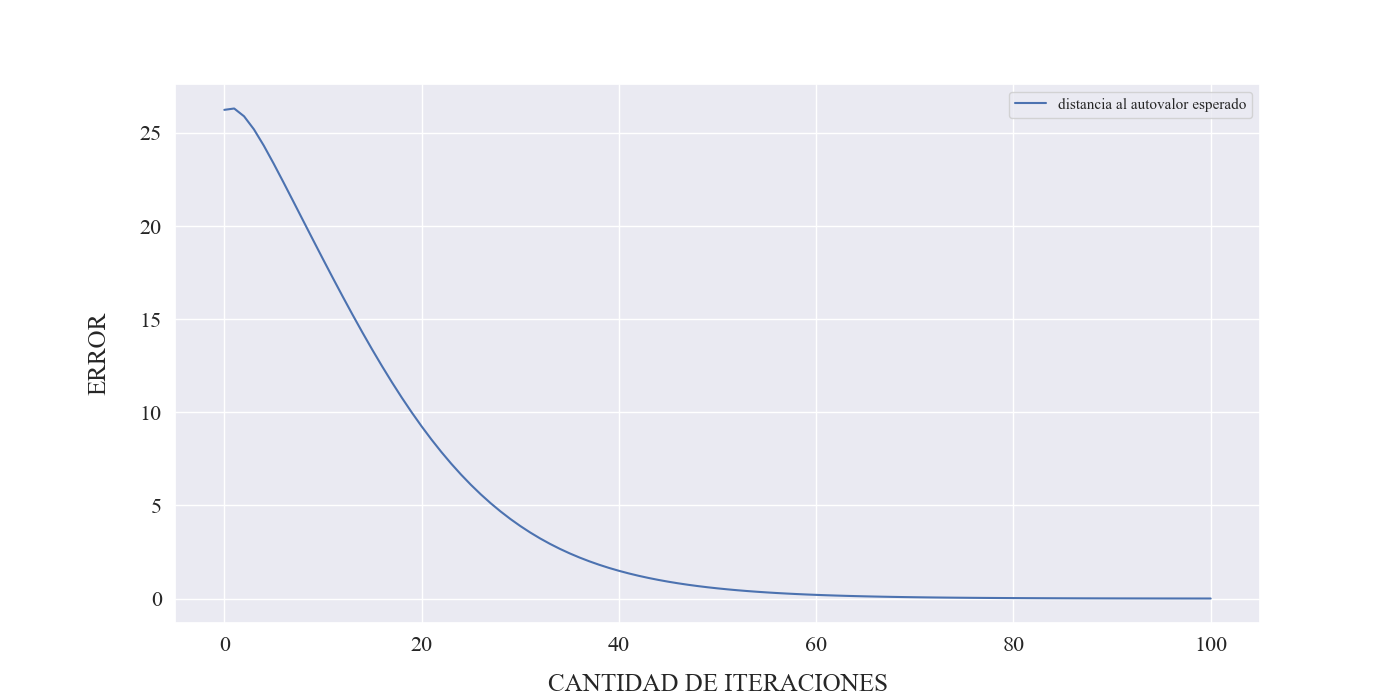
\includegraphics[scale=0.45]{files/src/.media/op_autovalor_repetido.png}
    \caption{Se eligió una matriz de $20 \times 20$ con base de autovectores y dos autovalores dominantes ($\lambda_1 = \lambda_2 = 20$). En cada iteración del método de la potencia medimos el error absoluto $||20 - \bar{\lambda}||_2$. Se puede observar como, a medida que aumenta la cantidad de iteraciones, la distancia entre el autovalor y el esperado tiende a cero.}
    \label{fig:autovalor_repetido}
\end{figure}

\vspace{1em}
Cabe destacar que como $\sum_{i=1}^{k} c_i\ x_i$ es autovector para todo $c_i$ ($\exists c_i \neq 0$). Entonces cualquier combinación lineal de los $x_i$ va a ser un autovector, y por ende hay infinitos resultados posibles con norma igual a uno ---a diferencia del caso en el que todos los autovalores son diferentes en módulo, donde hay solo dos autovectores con norma uno---.

\vspace{1em}
Algo interesante a notar es que, por tomar $k$ par, pudimos asumir que $signo(\lambda_1)^k = (\frac{|\lambda_{1}|}{\lambda_{1}})^k = 1$. Si no fueramos a asumir esto, observamos que en las iteraciones pares el metodo converge a $\sum_{i=1}^{k} c_i\ x_i$, pero en las impares podría converger a $-\sum_{i=1}^{k} c_i\ x_i$. Ambos son autovectores válidos linealmente dependientes. Por lo que la restriccion de $k$ par no es necesaria para encontrar un autovector.

Sin embargo, teniendo en cuenta que el método depende de la distancia entre una iteración y su consecutiva, como en este caso el método oscila entre iteraciones pares e iteraciones impares, la distancia entre una iteración y su consecutiva no tendera a cero. En consecuencia, de no imponer esta restriccion, el método va a tener que que hacer el total de las iteraciones sin poder interrumpirse antes. 










\vspace{2em}
\subsubsection*{2. Método de la potencia para autovalores diferentes pero iguales en módulo} 

Si suponemos, en cambio, que $|\lambda_1| = ... = |\lambda_k|$, vemos que $(\frac{\lambda_i}{\lambda_1})^k = signo(\lambda_i)^k\ \ \forall i: 1\ ...\ k$, y la ecuación (\ref{eq_potencia}.) se comporta de la siguiente manera:

\begin{equation*}
    \lim_{k \to \infty} b_k = \sum_{i=1}^{k} signo(\lambda_i)^k\ c_i\ x_i = \sum_{i=1}^{k} d_i\ x_i  
\end{equation*}

\vspace{1em}
\noindent donde $d_i = signo(\lambda_i)^k\ c_i$.


% \begin{align}
%     let \ norm \ :&= \ ||\sum_{i=1}^{n} a_i \ \lambda_{i}^{k} \ x_i||_2 \\
%     \lim_{k \to \infty} y_k &= \frac{\sum_{i=1}^{n} a_i \ \lambda_{i}^{k} \ x_i }{norm} \\ 
%     \lim_{k \to \infty} y_k &= \frac{(\sum_{i=1}^{n} a_i \ \lambda_{i}^{k} \ x_i) / \lambda_{1}^{k}}{norm / \lambda_{1}^{k}} \\
%     let \ b_i \ :&= \ \frac{a_i}{norm / \lambda_{1}^{k}} \\
%     \lim_{k \to \infty} y_k &= \sum_{i=1}^{n} b_i \ \frac{\lambda_{i}^{k}}{\lambda_{1}^{k}} \ x_i \\
%     \lim_{k \to \infty} y_k &= b_1 x_1 + b_2 \ \frac{\lambda_{2}^{k}}{\lambda_{1}^{k}} \ x_2 \\
%     \lim_{k \to \infty} y_k &= b_1 x_1 + b_2 \ sign(\lambda_{2}^{k}) \ x_2 
% \end{align}

\vspace{1em}
\noindent Notamos que este vector oscilará si k es impar, ya que dependerá del signo de cada autovalor dominante. Lo que es más, de tomar la subsecuencia convergente para $k$ par, este no necesariamente será un autovector. Vemos que para $d_1\ ...\ d_k$ arbitrarios ($\exists d_i \neq 0)$:

\begin{equation*}
    \mathbf{A} \sum_{i=1}^{k} d_i\ x_i = \sum_{i=1}^{k} \mathbf{A} d_i\ x_i = \sum_{i=1}^{k} \lambda_i\ d_i\ x_i 
\end{equation*}

\vspace{1em} 
\noindent Si existe al menos un $\lambda_j$ negativo, $1 \leq j \leq k$, entonces:

\begin{equation*}
    \sum_{i=1}^{k} \lambda_i\ d_i\ x_i = \lambda_1 \sum_{i = 1,\ i \neq j}^{k} d_i\ x_i - |\lambda_j|\ d_j\ x_j = \lambda_1 (\sum_{i = 1,\ i \neq j}^{k} d_i\ x_i - d_j\ x_j)
\end{equation*}

\vspace{1em} 
\noindent pero:

\begin{equation*}
    \sum_{i=1}^{k} d_i\ x_i \neq \sum_{i = 1,\ i \neq j}^{k} d_i\ x_i - d_j\ x_j
\end{equation*}

\vspace{1em}
\noindent por lo que el método de la potencia no converge a un autovector. 
Un ejemplo de esto se puede observar en el gráfico (\ref{fig:oscilante}.).

\vspace{1em}
Con este resultado en mente observamos que en caso de computar la suma entre las últimas dos iteraciones del método de la potencia, para $k$ par lo suficientemente grande, obtendríamos lo siguiente:

\vspace{1em}
\begin{align*}
    b_k &= \sum_{i=1}^{k} c_i\ x_i \\
    b_{k+1} &= \sum_{i=1}^{k} d_i\ x_i = \sum_{i: \lambda_i > 0}^{k} c_i\ x_i - \sum_{i: \lambda_i < 0}^{k} c_i\ x_i \\ 
    b_k + b_{k+1} &= \sum_{i=1}^{k} c_i\ x_i + \sum_{i: \lambda_i > 0}^{k} c_i\ x_i - \sum_{i: \lambda_i < 0}^{k} c_i\ x_i   \\ 
    b_k + b_{k+1} &= 2 \sum_{i: \lambda_i > 0}^{k} c_i\ x_i
\end{align*}

\vspace{1em}
Es decir, estaríamos en la condición del caso anterior, por lo que este valor sí converge al autovector asociado a $\lambda_1$.

\begin{figure}[!htbp]
    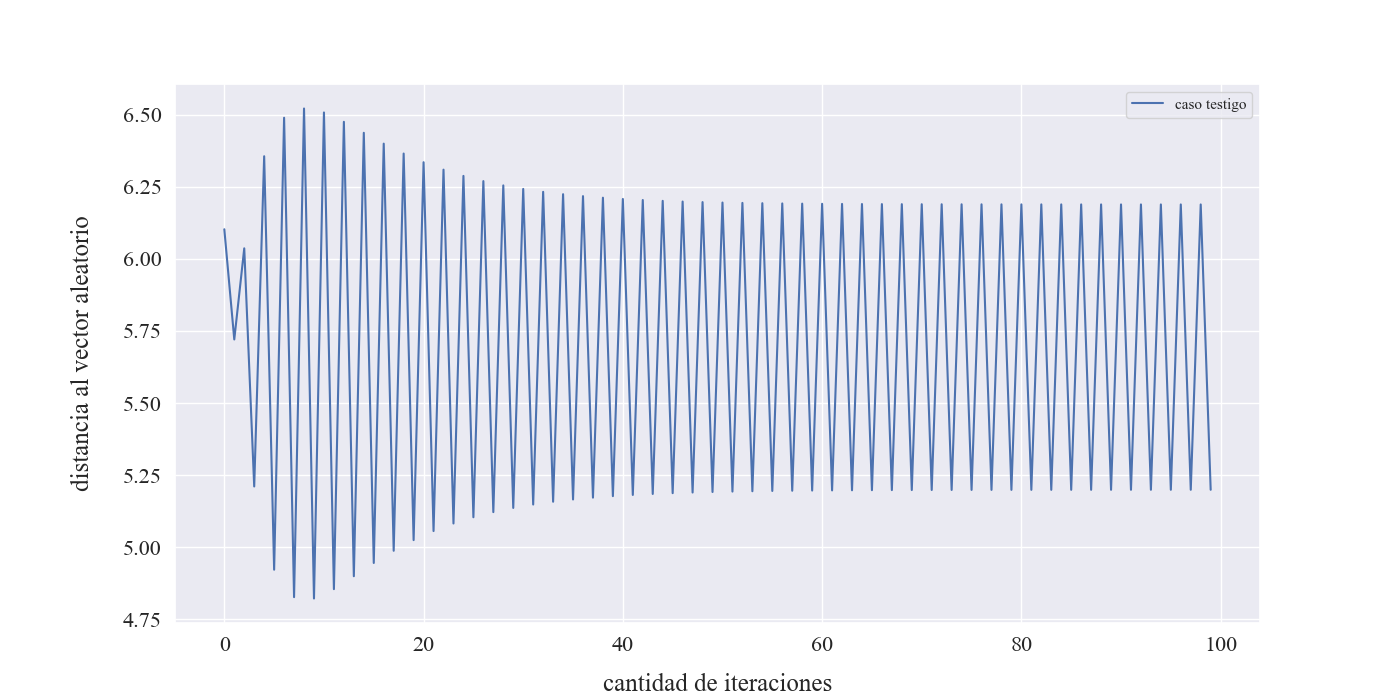
\includegraphics[scale=0.45]{files/src/.media/op_oscilante.png}
    \caption{Se eligió una matriz de $20 \times 20$ con base de autovectores y dos autovalores dominantes $\lambda_1 = 20$, $\lambda_2 = -20$. Además se seleccionó un vector aleatorio constante normalizado $v$ y en cada iteración del método de la potencia calculamos la distancia $||v - y_k||_2$. Se puede apreciar como la distancia a $v$ oscila entre las iteraciones pares e impares.}
    \label{fig:oscilante}
\end{figure}

\vspace{1em}

\vspace{1em}
Observamos que se podría calcular la resta para obtener otro autovector (asociado $\sum_{i: \lambda_i < 0}^{k} c_i\ x_i$). Como la deflacíon asume que el método de la potencia encuentra de a un autovector por llamado, consideramos que no vale la pena modificar el algoritmo para este caso puntual.


\vspace{2em}
\subsubsection*{3. Una extensión del método de la potencia} Con este resultado en mente planteamos el siguiente algoritmo como alternativa para el método de la potencia \textit{monte carlo}.

\vspace{1em}
\lstinputlisting[mathescape=true, escapechar=@, language=pseudo, label=potencia_modificada, caption={Pseudocódigo mostrando la alternativa a la potencia que soluciona cuando hay autovalores repetidos}]{files/src/.code/potencia_modificada.pseudo}

\vspace{1em}
Dada una matriz inicial cuyos autovalores pertenecen a los reales, este nuevo algoritmo permite relajar las restricciones del método original.

% \vspace{1em}

% \begin{large}  
%     \textbf{¿Cuantás iteraciones del método de la potencia son necesarias para que converja según el tamaño de la matriz?}
% \end{large}  

% \vspace{1em}
% Para responder esta pregunta experimentamos de la siguiente manera:

% \vspace{1em}
% \lstinputlisting[language=pseudo, label=experimento_iteraciones, caption={Experimento para entender la complejidad del método de la potencia}]{files/src/.code/experimento_iteraciones.pseudo}
% \vspace{1em}

% \vspace{1em}
% \begin{figure}[!htbp]
%     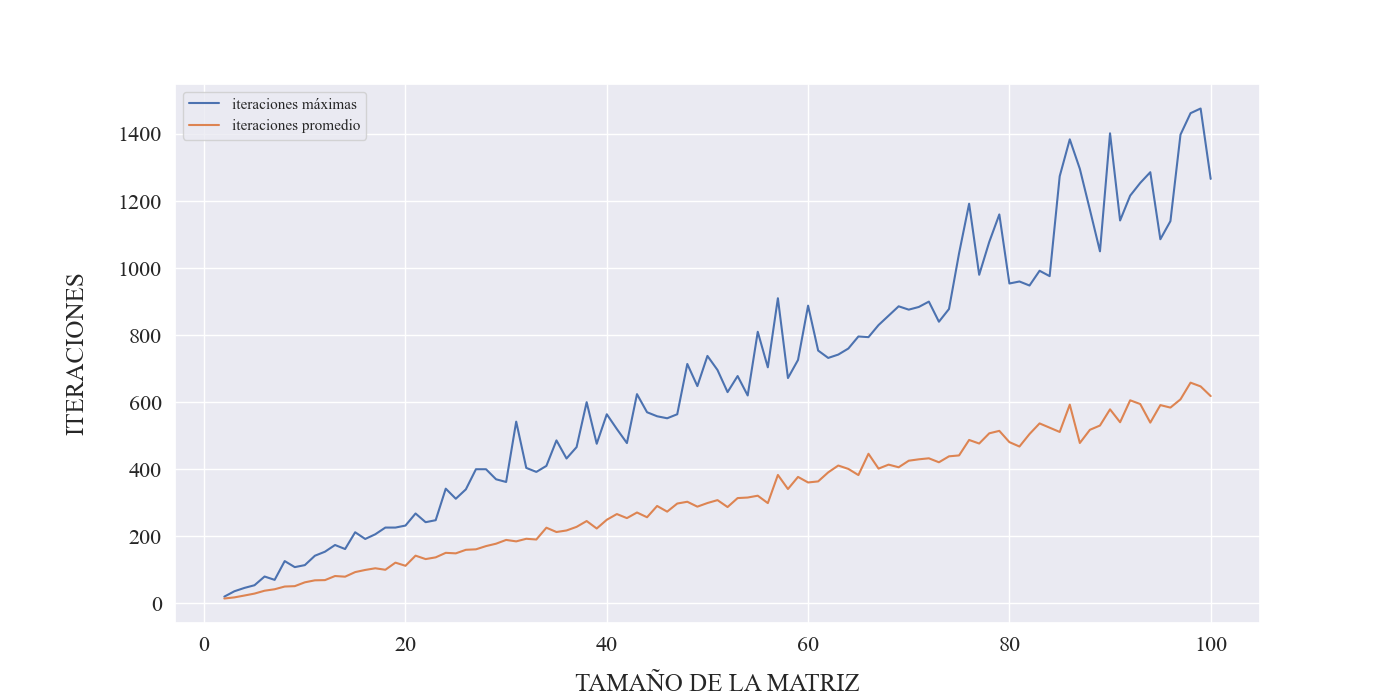
\includegraphics[scale=0.45]{files/src/.media/op_experimento_iteraciones.png}
%     \caption{Por cada i del algoritmo mostrado arriba se calculó el promedio de las iteraciones y la cantidad máxima de iteraciones.}
%     \label{fig:iteraciones}
% \end{figure}
% \vspace{1em}

% Se puede apreciar en el gráfico (\ref{fig:iteraciones}) que ambas curvas asemejan ser funciones lineales, deducimos que la cantidad de iteraciones necesarias para que el método de la potencia converja es lineal con respecto al tamaño de la matriz inicial.
% Este resultado, sumado a que la complejidad del método de la potencia es $O(N^2 * iteraciones)$ nos permite concluir que la complejidad promedio del método de la potencia es $\Theta(N^3)$